 %Version 3.1 December 2024
% See section 11 of the User Manual for version history
%
%%%%%%%%%%%%%%%%%%%%%%%%%%%%%%%%%%%%%%%%%%%%%%%%%%%%%%%%%%%%%%%%%%%%%%
%%                                                                 %%
%% Please do not use \input{...} to include other tex files.       %%
%% Submit your LaTeX manuscript as one .tex document.              %%
%%                                                                 %%
%% All additional figures and files should be attached             %%
%% separately and not embedded in the \TeX\ document itself.       %%
%%                                                                 %%
%%%%%%%%%%%%%%%%%%%%%%%%%%%%%%%%%%%%%%%%%%%%%%%%%%%%%%%%%%%%%%%%%%%%%

%%\documentclass[referee,sn-basic]{sn-jnl}% referee option is meant for double line spacing

%%=======================================================%%
%% to print line numbers in the margin use lineno option %%
%%=======================================================%%

%%\documentclass[lineno,pdflatex,sn-basic]{sn-jnl}% Basic Springer Nature Reference Style/Chemistry Reference Style

%%=========================================================================================%%
%% the documentclass is set to pdflatex as default. You can delete it if not appropriate.  %%
%%=========================================================================================%%

%%\documentclass[sn-basic]{sn-jnl}% Basic Springer Nature Reference Style/Chemistry Reference Style

%%Note: the following reference styles support Namedate and Numbered referencing. By default the style follows the most common style. To switch between the options you can add or remove “Numbered” in the optional parenthesis. 
%%The option is available for: sn-basic.bst, sn-chicago.bst%  
 
%%\documentclass[pdflatex,sn-nature]{sn-jnl}% Style for submissions to Nature Portfolio journals
%%\documentclass[pdflatex,sn-basic]{sn-jnl}% Basic Springer Nature Reference Style/Chemistry Reference Style
\documentclass[pdflatex,sn-mathphys-num]{sn-jnl}% Math and Physical Sciences Numbered Reference Style
%%\documentclass[pdflatex,sn-mathphys-ay]{sn-jnl}% Math and Physical Sciences Author Year Reference Style
%%\documentclass[pdflatex,sn-aps]{sn-jnl}% American Physical Society (APS) Reference Style
%%\documentclass[pdflatex,sn-vancouver-num]{sn-jnl}% Vancouver Numbered Reference Style
%%\documentclass[pdflatex,sn-vancouver-ay]{sn-jnl}% Vancouver Author Year Reference Style
%%\documentclass[pdflatex,sn-apa]{sn-jnl}% APA Reference Style
%%\documentclass[pdflatex,sn-chicago]{sn-jnl}% Chicago-based Humanities Reference Style

%%%% Standard Packages
%%<additional latex packages if required can be included here>

\usepackage{graphicx}%
\usepackage{multirow}%
\usepackage{amsmath,amssymb,amsfonts}%
\usepackage{amsthm}%
\usepackage{fix-cm}
\usepackage{mathrsfs}%
\usepackage[title]{appendix}%
\usepackage{xcolor}%
\usepackage{textcomp}%
\usepackage{manyfoot}%
\usepackage{booktabs}%
\usepackage{algorithm}%
\usepackage{algpseudocode}%
\usepackage{listings}%
\usepackage{cite}
\usepackage{tikz}
\usetikzlibrary{shapes,arrows,positioning}
\usepackage{float}      % 
\usepackage{booktabs}   % 
%%%%

%%%%%=============================================================================%%%%
%%%%  Remarks: This template is provided to aid authors with the preparation
%%%%  of original research articles intended for submission to journals published 
%%%%  by Springer Nature. The guidance has been prepared in partnership with 
%%%%  production teams to conform to Springer Nature technical requirements. 
%%%%  Editorial and presentation requirements differ among journal portfolios and 
%%%%  research disciplines. You may find sections in this template are irrelevant 
%%%%  to your work and are empowered to omit any such section if allowed by the 
%%%%  journal you intend to submit to. The submission guidelines and policies 
%%%%  of the journal take precedence. A detailed User Manual is available in the 
%%%%  template package for technical guidance.
%%%%%=============================================================================%%%%

%% as per the requirement new theorem styles can be included as shown below
\theoremstyle{thmstyleone}%
\newtheorem{theorem}{Theorem}%  meant for continuous numbers
%%\newtheorem{theorem}{Theorem}[section]% meant for sectionwise numbers
%% optional argument [theorem] produces theorem numbering sequence instead of independent numbers for Proposition
\newtheorem{proposition}[theorem]{Proposition}% 
%%\newtheorem{proposition}{Proposition}% to get separate numbers for theorem and proposition etc.

\theoremstyle{thmstyletwo}%
\newtheorem{example}{Example}%
\newtheorem{remark}{Remark}%

\theoremstyle{thmstylethree}%
\newtheorem{definition}{Definition}%

\raggedbottom
%%\unnumbered% uncomment this for unnumbered level heads

\begin{document}

\title[Article Title]{Article Title}

%%=============================================================%%
%% GivenName	-> \fnm{Joergen W.}
%% Particle	-> \spfx{van der} -> surname prefix
%% FamilyName	-> \sur{Ploeg}
%% Suffix	-> \sfx{IV}
%% \author*[1,2]{\fnm{Joergen W.} \spfx{van der} \sur{Ploeg} 
%%  \sfx{IV}}\email{iauthor@gmail.com}
%%=============================================================%%

\author*[1,2]{\fnm{First} \sur{Author}}\email{iauthor@gmail.com}

\author[2,3]{\fnm{Second} \sur{Author}}\email{iiauthor@gmail.com}
\equalcont{These authors contributed equally to this work.}

\author[1,2]{\fnm{Third} \sur{Author}}\email{iiiauthor@gmail.com}
\equalcont{These authors contributed equally to this work.}

\affil*[1]{\orgdiv{Department}, \orgname{Organization}, \orgaddress{\street{Street}, \city{City}, \postcode{100190}, \state{State}, \country{Country}}}

\affil[2]{\orgdiv{Department}, \orgname{Organization}, \orgaddress{\street{Street}, \city{City}, \postcode{10587}, \state{State}, \country{Country}}}

\affil[3]{\orgdiv{Department}, \orgname{Organization}, \orgaddress{\street{Street}, \city{City}, \postcode{610101}, \state{State}, \country{Country}}}

%%==================================%%
%% Sample for unstructured abstract %%
%%==================================%%

\abstract{Unmanned Aerial Vehicles (UAVs) rely on the MAVLink protocol for continuous exchange of control commands, telemetry, and mission data between onboard systems and ground control stations. Under real-time operating conditions, a large number of MAVLink messages are generated every second, which can lead to network congestion, increased latency, and delayed delivery of safety-critical messages in bandwidth-constrained environments. In addition, repeated or redundant telemetry messages further increase channel load without providing significant operational benefit.

This paper proposes a machine learning--based message prioritization and congestion mitigation framework for MAVLink-enabled UAV communication systems. A lightweight ML model is deployed at the UAV edge to dynamically assign priority levels to MAVLink messages based on a feature vector 
$\mathbf{x} = [m_t, p_s, f_r, s_u, c_m]$, 
where $m_t$ denotes message type, $p_s$ the payload size, $f_r$ the transmission frequency, $s_u$ the system state, and $c_m$ the mission context. The model learns a mapping $f(\mathbf{x}) \rightarrow \pi$, where $\pi$ represents the inferred priority class. 

To address congestion, the framework monitors the message arrival rate $\lambda$ and selectively suppresses repeated or low-impact messages when $\lambda$ exceeds a predefined threshold $\lambda_{th}$. Priority-aware queue management ensures that control, navigation, and safety-critical messages are transmitted with minimal delay, while non-critical messages are deferred or discarded during high-load periods. The proposed approach preserves MAVLink backward compatibility by avoiding modifications to the message format or additional protocol overhead.

Experimental evaluation shows that the proposed ML-driven prioritization significantly reduces end-to-end latency and packet loss for high-priority messages, while maintaining low computational and memory overhead suitable for resource-constrained UAV platforms. The results demonstrate that integrating intelligent prioritization with redundancy elimination improves the robustness and real-time performance of UAV communication systems.}



\keywords{UAV Communication Systems, MAVLink, Traffic Prioritization, Edge Intelligence}


%%\pacs[JEL Classification]{D8, H51}

%%\pacs[MSC Classification]{35A01, 65L10, 65L12, 65L20, 65L70}

\maketitle

\section{ Introduction }
\subsection{ Background and Motivation }
Un-Manned Aerial Vehicles are being used in many areas like communication, surveilance, environmental monitoring, disaster management, rescue operations etc that is clearly stated in \citet{ghamari2022unmanned}. In many of the cases, one UAV alone cannot manage all the work, so a group of UAV's are deployed and all are collaborated by exchanging messages, and forms UAV Ad Hoc Network (UAANET) \citet{rovira2022review} . However, due to high mobility, limited bandwidth, and other dynamic conditions (from \citet{nawaz2021uav}), some communication packets get dropped/missed which makes reliable communication remains a significant challenge while using UAV's in different situations.\\
\\
Furthermore, UAANETs differ significantly from traditional mobile ad hoc networks due to their three-dimensional mobility, higher node speeds, and rapidly changing network topology(\citet{amponis2021survey}). These characteristics make link stability highly unpredictable and routing paths short-lived, leading to frequent route failures and retransmissions. As the number of UAVs participating in the network increases, the communication overhead also grows, which can further strain the limited wireless bandwidth(\citet{yang2022improved}). Consequently, efficient traffic management becomes essential to prevent network congestion and ensure reliable inter-UAV communication in highly dynamic operating environments.\\
\\
 MAVLink became very popular for transferring the message packets between the UAVs(\citet{cordill2025comprehensive}). Despite its popularity, MAVLink rely on static or manually configured message transmission rates which may not be suitable for dynamic conditions(\citet{lee2021enabling}) and in some cases congestion may arise in the network where the inflow of the message packets are more than the total bandwidth of the network for communication, as a result some the packets get dropped(\citet{anwekar2023analysis}).\\ 
\\
In congested network scenarios, packet dropping alone is not an effective solution, as it leads to unnecessary retransmissions, increased delay, and inefficient use of network resources(\citet{anwekar2023analysis}). This problem becomes more critical in UAV networks where communication links are often unstable and energy resources are limited. Studies have shown that proactive congestion control techniques, which regulate traffic flow before buffer overflow occurs, can significantly reduce packet loss and improve overall network performance. In particular, rate-based congestion control approaches are more suitable for UAV networks, as they dynamically adapt the traffic generation rate to current network conditions(\citet{verma2024adaptive}).\\
\\
 In addition, UAV communication involves heterogeneous message types such as command and control messages, telemetry data, navigation information, and sensor payload data (\citet{cordill2025comprehensive}), each having different priority and delay requirements. Treating all messages with the same transmission rate and priority can further aggravate congestion, especially during mission-critical operations where timely delivery of control messages is essential(\citet{ribeiro2021communication}). Recent studies emphasize that adaptive communication mechanisms which consider message importance and real-time network conditions can significantly improve Quality of Service (QoS) and overall system reliability in UAV Ad Hoc Networks(\citet{buenrostro2023prioritization}). Therefore, incorporating congestion-aware and priority-sensitive message rate control mechanisms becomes a crucial requirement for ensuring robust and reliable UAV communication.\\
 \\
 Moreover, the dynamic nature of UAV missions implies that network conditions can vary significantly over time due to changes in UAV density, mobility patterns, and communication range. During critical mission phases such as takeoff, formation flying, collision avoidance, or emergency response, the volume of control and telemetry messages may increase sharply, further intensifying network congestion(\citet{mohsan2023unmanned}). Static communication strategies are unable to accommodate such temporal traffic variations. Recent studies indicate that adaptive and context-aware communication mechanisms(\citet{rovira2022review}), which continuously monitor network conditions and adjust transmission behavior accordingly, are essential for maintaining reliable and scalable UAV communications.\\
 
This packet loss can lead to poor Quality of Service (QoS).So these limitations motivates to work and propose adaptive rate control algorithm in UAV Communicaiton.







\subsection{ Problem Statement }
In UAANET, there are different types of messages like command messages, telementry messages, sensor data packets, Location update messages etc. these are being transmitted by static transmission rates.
    But, in some cases congestion can occur in the UAV Network where the incoming messages are more when compared to the bandwidth of the network and as a result while transmitting the message packets, few will get dropped. As a result the QoS will get effected and failure of task and missions.

Current solutions mainly focus on packet scheduling and messaging routing. while message rate control remains unexplored comparitvely. There is lack of mechanism that dynamically regulates the rate flow based on the congestion.




\subsection{ Research Objectives and Contributions }
The primary objective of this research is to create and evaluate congestion aware rate control mechanism for MAVLink based communication.The proposed approach helps us to adjust the message transmission rate dynamically based on the congestion present in the network which will directly increase the Quality of Service (QoS). This ensure the improvised bandwidth utilization and imporves reliability on MAVLink.

Key Contributions are:\\
    \hspace*{2em}1. Classificaiton of messages using Machine Learning Model and prioritising them.\\
    \hspace*{2em}2. Heuristic rate aware congestion control Algorithm.\\
    \hspace*{2em}3. Message scheduling Algorithm in queue before transmission.\\



\begin{figure}[h]
\centering

\includegraphics[width=0.9\columnwidth]{fifomodel.png}
\caption{FIFO based Network Model}
\label{fig:my_image}
\end{figure}

\begin{figure}[h]
\centering

\includegraphics[width=0.9\columnwidth]{MLBasedHeuristicModel.drawio.png}
\caption{ML based Heuristic Network Model}
\label{fig:my_image}
\end{figure}





\subsection{ Organization of the Paper }




\section{Related Work}

\subsection{Existing Approaches and Techniques}

UAV communication networks have received significant attention in recent years due to their growing adoption in civil, industrial, and defense applications. A comprehensive review by \citet{ghamari2022unmanned} discusses UAV communication architectures, spectrum challenges, interference management, and reliability requirements in civil deployments. The study emphasizes that UAV communication must operate under strict latency, reliability, and bandwidth constraints, particularly during mission-critical operations such as disaster monitoring and emergency response.

From a networking perspective, Flying Ad Hoc Networks (FANETs) and UAV Ad Hoc Networks (UAANETs) exhibit unique characteristics including high node mobility, frequent topology changes, intermittent connectivity, and three-dimensional movement. These properties distinguish them from traditional MANETs and VANETs. A cross-layer survey by \citet{amponis2021survey} highlights the importance of joint optimization across physical, MAC, and network layers to maintain reliable communication in dynamic UAV environments. Similarly, \citet{nawaz2021uav} identifies bandwidth limitation, packet loss, congestion, and routing instability as major challenges affecting UAV communication performance.

Routing strategies have been extensively studied to address link instability. AI-enabled routing approaches reviewed by \citet{rovira2022review} demonstrate that machine learning and reinforcement learning techniques can improve route selection in highly dynamic UAV networks. Adaptive routing designs proposed by \citet{zhang2022adaptive} and extended in \citet{zhang2023adaptive} use prediction-based mechanisms to estimate link stability and proactively select reliable paths. These approaches improve network-layer reliability; however, they primarily focus on routing optimization rather than application-layer traffic regulation or congestion-aware rate adaptation.

Clustering techniques have also been explored to reduce communication overhead. The weighted and location-based clustering scheme proposed by \citet{yang2022improved} enhances network scalability by organizing UAVs into structured clusters. Although clustering reduces routing overhead, it does not directly regulate message transmission rates or prioritize application-layer packets such as MAVLink messages.

At the application layer, MAVLink has emerged as the de facto communication protocol for UAV systems. The survey by \citet{koubaa2019micro} provides a detailed explanation of MAVLink architecture, message structure, serialization format, and operational characteristics. MAVLink supports periodic and event-driven messages, including heartbeat, telemetry, command, and mission updates. Despite its lightweight design, MAVLink relies on statically configured transmission intervals, which may lead to excessive channel utilization under high-load conditions. Furthermore, \citet{cordill2025comprehensive} discusses security and privacy issues in UAV systems and highlights that communication overload and congestion can amplify security vulnerabilities by increasing retransmissions and attack surfaces.

To enhance reliability, \citet{lee2021enabling} propose transmitting duplicated control packets across multiple protocols and paths to ensure UAV control robustness. While duplication improves reliability, it may increase network load and aggravate congestion under bandwidth constraints. Similarly, the communication interface manager proposed by \citet{ribeiro2021communication} enables heterogeneous interface selection to improve throughput and reduce latency. However, these methods focus on path diversity and interface optimization rather than adaptive rate regulation.

Congestion control has been widely studied in wireless sensor and IoT networks. The rate-aware congestion control mechanism proposed by \citet{grover2022rate} dynamically adjusts packet transmission rates based on network load metrics such as buffer occupancy and packet loss. Their approach effectively reduces packet drops and improves throughput in wireless sensor networks. Likewise, \citet{verma2024adaptive} introduce a one-way delay–based adaptive congestion control technique for IoT networks, which proactively regulates traffic before severe congestion occurs. Although these techniques demonstrate the effectiveness of rate-based adaptation, they treat packets uniformly and do not consider message semantics or priority differentiation.

In UAV-specific environments, \citet{anwekar2023analysis} analyze congestion control techniques in FANETs and demonstrate that uncontrolled traffic inflow significantly degrades Quality of Service (QoS). The study confirms that congestion-aware rate adaptation can improve reliability and communication stability. Additionally, \citet{buenrostro2023prioritization} propose a prioritization-driven cross-layer congestion control mechanism in Internet of Medical Things (IoMT) networks, highlighting the importance of semantic packet prioritization in delay-sensitive environments. However, their work is not tailored to MAVLink-based UAV systems.

Priority-based scheduling approaches have also been proposed in UAV networks. The message scheduling scheme introduced by \citet{li2018prioritizing} ensures timely delivery of critical UAV messages by assigning predefined priority levels. Similarly, the dynamic super round-based distributed scheduling algorithm proposed by \citet{halder2022dynamic} enhances coordination efficiency in multi-UAV systems by organizing communication into structured rounds. More recently, \citet{yang2025intelligent} propose an intelligent queue scheduling mechanism for SPMA-based UAV networks, which improves packet handling efficiency at the MAC layer.

Although these scheduling-based methods enhance timeliness and reliability, they primarily operate at MAC or network layers and depend on predefined priority rules. They do not integrate adaptive learning-based classification at the application layer, nor do they dynamically regulate MAVLink transmission rates based on congestion levels.

Furthermore, \citet{mohsan2023unmanned} discuss open challenges in UAV systems, emphasizing scalability, congestion management, and adaptive communication as key research directions. The authors highlight that future UAV networks must incorporate intelligent and context-aware mechanisms to handle increasing traffic loads and mission complexity.

Overall, prior research has explored routing optimization, clustering, interface management, congestion control, and priority scheduling independently. However, limited work integrates machine learning–based message classification with congestion-aware rate control specifically for MAVLink-enabled UAV communication systems.

\subsection{Comparative Analysis of Prior Studies}

Existing literature can be categorized into five major groups: (i) UAV communication surveys and architectural studies, (ii) routing and clustering mechanisms, (iii) reliability enhancement techniques, (iv) congestion control approaches, and (v) priority-based scheduling schemes.

Survey works such as \citet{ghamari2022unmanned}, \citet{nawaz2021uav}, and \citet{mohsan2023unmanned} provide comprehensive insights into UAV communication challenges, including spectrum scarcity, dynamic topology, and congestion. While these studies outline the need for adaptive mechanisms, they do not propose concrete application-layer rate control strategies.

Routing-focused studies \citep{rovira2022review,zhang2022adaptive,zhang2023adaptive} improve path stability using prediction and AI-based techniques. Clustering methods such as \citet{yang2022improved} reduce routing overhead and enhance scalability. However, these approaches operate primarily at the network layer and do not regulate the generation rate of MAVLink messages.

Reliability-enhancing solutions, including multi-path duplication \citep{lee2021enabling} and heterogeneous interface management \citep{ribeiro2021communication}, improve communication robustness but may increase traffic load, potentially worsening congestion.

Congestion control mechanisms proposed for wireless sensor and IoT networks \citep{grover2022rate,verma2024adaptive} demonstrate the effectiveness of rate adaptation based on congestion metrics. FANET-specific analyses \citep{anwekar2023analysis} confirm that congestion severely impacts QoS. However, these approaches lack semantic awareness and do not distinguish between critical and non-critical UAV messages.

Priority-based scheduling techniques \citep{li2018prioritizing,halder2022dynamic,yang2025intelligent} ensure timely transmission of important packets but rely on predefined priority classes and do not integrate machine learning for dynamic classification. Moreover, they focus on scheduling rather than controlling the rate at which messages are generated and transmitted.

The MAVLink survey by \citet{koubaa2019micro} identifies static transmission configuration as a limitation but does not propose adaptive congestion-aware mechanisms. Security-focused analysis by \citet{cordill2025comprehensive} further indicates that communication inefficiencies can exacerbate vulnerabilities, reinforcing the need for intelligent traffic management.

Thus, while substantial progress has been made across routing, scheduling, and congestion control domains, a unified framework that combines machine learning–based message prioritization with congestion-aware rate regulation at the MAVLink application layer remains largely unexplored.

\subsection{Research Gaps and Limitations}

Despite extensive research, several critical gaps remain in the literature:

\begin{itemize}
    \item \textbf{Lack of Application-Layer Adaptation:} Most routing and clustering techniques \citep{zhang2022adaptive,yang2022improved} operate at lower layers and do not control MAVLink message transmission rates.
    
    \item \textbf{Static MAVLink Configuration:} MAVLink commonly uses predefined transmission intervals \citep{koubaa2019micro}, which may lead to congestion under dynamic traffic conditions.
    
    \item \textbf{Uniform Treatment of Packets:} Congestion control mechanisms \citep{grover2022rate,verma2024adaptive} treat packets equally without considering semantic importance.
    
    \item \textbf{Predefined Priority Rules:} Scheduling-based approaches \citep{li2018prioritizing,yang2025intelligent} rely on static priority assignments rather than adaptive learning-based classification.
    
    \item \textbf{Limited Integration of ML with Rate Control:} Although AI-based routing \citep{rovira2022review} has been explored, integrating machine learning for message-level prioritization combined with congestion-aware rate control remains insufficiently addressed.
\end{itemize}

Therefore, there is a clear need for an integrated framework that (i) classifies MAVLink messages dynamically using machine learning, (ii) estimates congestion using measurable network parameters, and (iii) regulates transmission rates according to both congestion severity and message priority. The proposed work addresses this gap by introducing a machine learning–based message prioritization mechanism combined with heuristic congestion-aware rate adaptation while maintaining full MAVLink protocol compatibility.

\section{ System Model / Architecture }

\subsection{ End-to-End System Architecture Diagram }

The complete framework integrates three functional blocks: MAVLink message generation, ML-based semantic prioritization, and RL-based combined scheduling and aggregation. Figure~\ref{fig:system_architecture_flow} illustrates the data flow and decision pipeline.



This system architecture has been designed to ease the adaptive, congestion-receptive communication in Unmanned Aerial Vehicle Ad Hoc Networks (UAANETs) and be compatible with MAVLink-based UAV systems.
The architecture is modular and separates the message generation, message classification, congestion estimation and adaptive rate control.
This form of segregation also allows learning based elements to be flexibly integrated without need of altering the underlying MAVLink protocol.
This system operates in a distributed manner and is able to adapt fast to the dynamism of the network conditions a UAV communication environment often experiences.\\

\begin{figure*}[t]
\centering
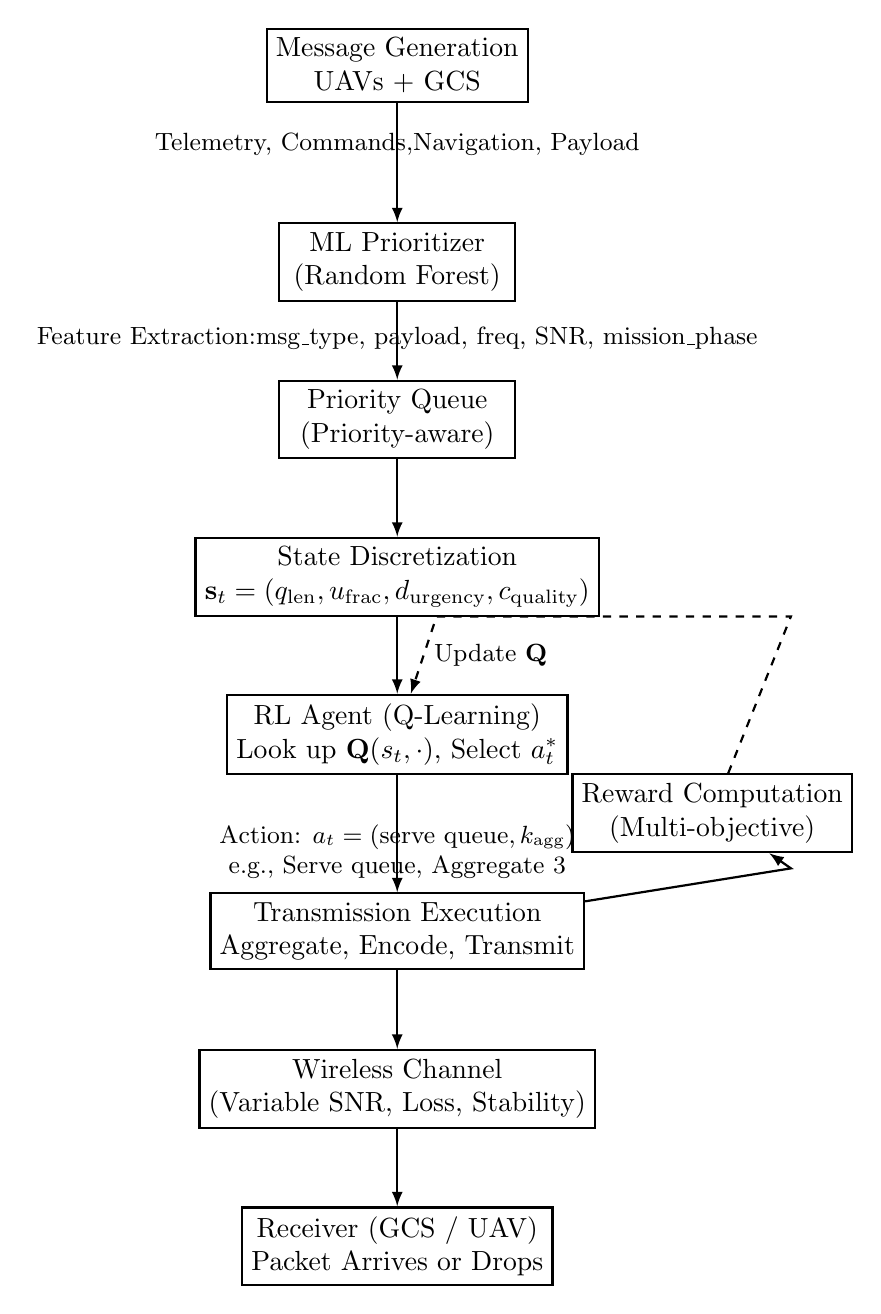
\begin{tikzpicture}[
  node distance=2cm,
  box/.style={rectangle, draw, thick, minimum width=3cm, minimum height=0.8cm, align=center},
  decision/.style={diamond, draw, thick, aspect=2, align=center},
  arrow/.style={->, thick, >=latex},
  label/.style={font=\small}
]
% Layer 1: Message Generation
\node[box] (gen) at (0, 8) {Message Generation\\UAVs + GCS};
% Messages flow
\node[label] (msg1) at (0, 7) {Telemetry, Commands,\\Navigation, Payload};

% Layer 2: ML-Based Prioritization
\node[box] (ml) at (0, 5.5) {ML Prioritizer\\(Random Forest)};
\draw[arrow] (gen) -- (ml);
\node[label, below=0.2cm of ml] {Feature Extraction:\\msg\_type, payload, freq, SNR, mission\_phase};
% Single priority queue
\node[box] (q) at (0, 3.5) {Priority Queue\\(Priority-aware)};
% Draw arrow from ML to queue
\draw[arrow] (ml) -- (q);
% Layer 3: State Discretization
\node[box] (state) at (0, 1.5) {State Discretization\\$\mathbf{s}_t = (q_{\text{len}}, u_{\text{frac}}, d_{\text{urgency}}, c_{\text{quality}})$};
% Draw arrow from queue to state
\draw[arrow] (q) -- (state);
% Layer 4: RL Agent
\node[box] (rl) at (0, -0.5) {RL Agent (Q-Learning)\\Look up $\mathbf{Q}(s_t, \cdot)$, Select $a_t^*$};
% Arrow from state to RL
\draw[arrow] (state) -- (rl);
% Add note showing action decoding
\node[below=0.5cm of rl, align=center, font=\small] {Action: $a_t = (\text{serve queue}, k_{\text{agg}})$\\e.g., Serve queue, Aggregate 3};
% Layer 5: Transmission
\node[box] (tx) at (0, -3) {Transmission Execution\\Aggregate, Encode, Transmit};
% Arrow from RL to TX
\draw[arrow] (rl) -- (tx);
% Feedback loop
\node[box] (reward) at (4, -1.5) {Reward Computation\\(Multi-objective)};
\draw[arrow] (tx) -- (5, -2.2) -- (reward);
% Update Q-table (dotted arrow back)
\draw[arrow, dashed] (reward) -- (5, 1) -- (0.5, 1) -- (rl) node[midway, right, font=\small] {Update $\mathbf{Q}$};
% Wireless channel
\node[box] (channel) at (0, -5) {Wireless Channel\\(Variable SNR, Loss, Stability)};
\draw[arrow] (tx) -- (channel);
% Receiver
\node[box] (rx) at (0, -7) {Receiver (GCS / UAV)\\Packet Arrives or Drops};
\draw[arrow] (channel) -- (rx);
\end{tikzpicture}
\caption{End-to-End Architecture: ML-Based Prioritization + RL-Based Scheduling and Aggregation Pipeline.}
\label{fig:system_architecture_flow}
\end{figure*}

Different streams of MAVLink messages are produced simultaneously from both UAVs and ground stations, such as command and control messages, telemetry messages, navigation messages and payload sensor messages. These messages vary in a great way with regard to importance, urgency and toleration of delay. In order to deal with such heterogeneity, the architecture proposes a message classification module, which is formed by Machine Learning, that will classify every message to one of the priority classes low, medium, and high according to the message attributes including the type, content, and operational relevance. ML model is trained offline on curated data sets.\\



Congestion estimation in the proposed architecture is performed using explicit network-level Parameters such as packet loss ratio, queue occupancy, and bandwidth utilization and they are continuously monitored to quantify the current congestion level of the network. These metrics are combined to derive a normalized congestion factor, which reflects the severity of congestion at a given time. This design choice ensures transparency, low computational overhead, and predictable behavior, which are critical for real-time UAV systems.\\


Based on the congestion factor and the priority class assigned by the ML model, the adaptive message rate control module dynamically regulates the transmission rates of different message baskets. High-priority messages experience minimal rate reduction to preserve reliable delivery of mission-critical information, while medium- and low-priority messages are progressively throttled as congestion increases. By decoupling message priority classification (ML-based) from congestion estimation (heuristic-based), the architecture achieves a balanced trade-off between intelligence and reliability, resulting in improved Quality of Service (QoS) and robust UAV communication under varying network conditions.

\subsection{ Network / Communication Model }

The network considered in this work is a UAV Ad Hoc Network (UAANET) consisting of multiple UAV nodes communicating over wireless links without fixed infrastructure. The UAVs operate in a shared and bandwidth-limited wireless medium, where network topology changes dynamically due to UAV mobility. Communication links are assumed to be unreliable and subject to packet loss, delay variation, and intermittent connectivity. Depending on mission requirements, communication may occur in single-hop or multi-hop fashion, with each UAV acting as both a data source and a relay node.\\

The communication between UAVs and the Ground Control Station is based on the MAVLink protocol, which operates at the application layer and typically uses UDP as the underlying transport protocol. MAVLink supports periodic and event-driven message exchanges, making it suitable for real-time UAV communication. In the proposed model, each UAV generates multiple concurrent MAVLink message streams, including heartbeat messages, telemetry data (e.g., GPS, IMU, battery status), navigation information, command and control messages, and high-bandwidth payload data such as camera frames etc.\\


Each MAVLink message is treated as an independent packet characterized by its message type, size, generation rate, and delay sensitivity. Messages are dynamically classified into three priority categories—high, medium, and low—using a Machine Learning–based classifier. High-priority messages include command and control and safety-critical information, medium-priority messages include telemetry and navigation data, and low-priority messages correspond to bandwidth-intensive or delay-tolerant payload data like temperature updates, battery status updates etc. This classification is performed before transmission and remains independent of the congestion estimation process.\\

Network congestion is modeled as a condition where the incoming message arrival rate exceeds the available communication capacity. Each UAV monitors local network indicators such as packet loss ratio, queue occupancy, and effective bandwidth utilization to assess the current congestion level. The estimated congestion level is calculated and then used by the adaptive rate control module to regulate the transmission rates of different message priority classes, ensuring reliable communication under dynamic network conditions.


\begin{figure}[h]
\centering
\resizebox{\columnwidth}{!}{%
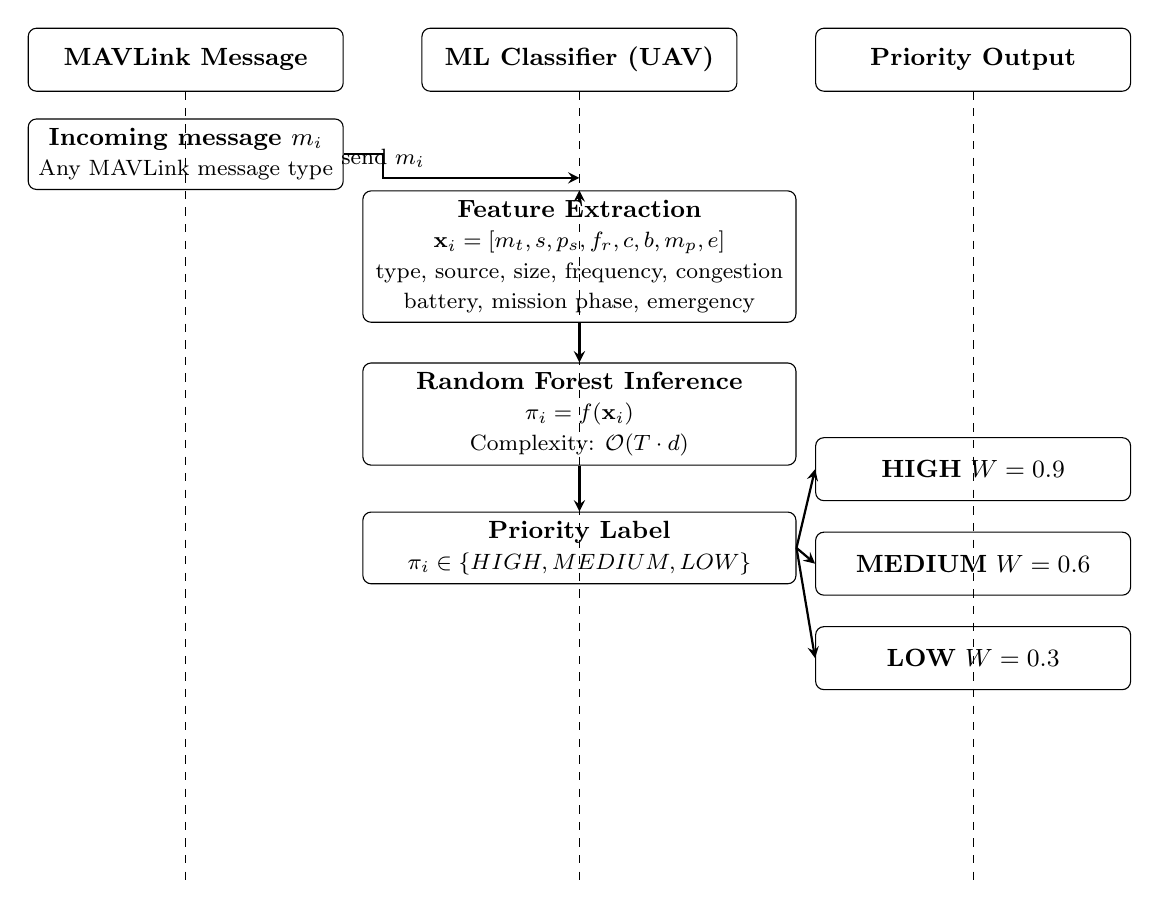
\begin{tikzpicture}[
    every node/.style={font=\small},
    box/.style={draw, rectangle, rounded corners=3pt, minimum width=4cm, minimum height=0.8cm, align=center},
    arr/.style={->, >=stealth, thick}
]

% Headers
\node[box] (msg) at (0, 0) {\textbf{MAVLink Message}};
\node[box] (ml)  at (5, 0) {\textbf{ML Classifier (UAV)}};
\node[box] (out) at (10, 0) {\textbf{Priority Output}};

% Lifelines (ONLY dotted lines now)
\draw[dashed] (0,  -0.4) -- (0,  -10.5);
\draw[dashed] (5,  -0.4) -- (5,  -10.5);
\draw[dashed] (10, -0.4) -- (10, -10.5);

% ❌ Removed this line:
% \draw[fill=white] (4.85, -0.4) rectangle (5.15, -8.5);

% Incoming message
\node[box] (incoming) at (0, -1.2)
{\textbf{Incoming message $m_i$}\\{\footnotesize Any MAVLink message type}};

% Arrow
\draw[arr] (incoming.east) -- ++(0.5,0) |- (5, -1.5)
node[midway, above, font=\footnotesize] {send $m_i$};

% Feature Extraction
\node[box, minimum width=5.5cm] (feat) at (5, -2.5)
{\textbf{Feature Extraction}\\
{\footnotesize $\mathbf{x}_i = [m_t, s, p_s, f_r, c, b, m_p, e]$}\\
{\footnotesize type, source, size, frequency, congestion}\\
{\footnotesize battery, mission phase, emergency}};

\draw[arr] (5, -1.8) -- (feat.north);

% Random Forest
\node[box, minimum width=5.5cm] (rf) at (5, -4.5)
{\textbf{Random Forest Inference}\\
{\footnotesize $\pi_i = f(\mathbf{x}_i)$}\\
{\footnotesize Complexity: $\mathcal{O}(T \cdot d)$}};

\draw[arr] (feat.south) -- (rf.north);

% Label
\node[box, minimum width=5.5cm] (label) at (5, -6.2)
{\textbf{Priority Label}\\
{\footnotesize $\pi_i \in \{HIGH, MEDIUM, LOW\}$}};

\draw[arr] (rf.south) -- (label.north);

% Outputs
\node[box] (high) at (10, -5.2) {\textbf{HIGH} $W=0.9$};
\node[box] (med)  at (10, -6.4) {\textbf{MEDIUM} $W=0.6$};
\node[box] (low)  at (10, -7.6) {\textbf{LOW} $W=0.3$};

\draw[arr] (label.east) -- (high.west);
\draw[arr] (label.east) -- (med.west);
\draw[arr] (label.east) -- (low.west);

\end{tikzpicture}%
}
\caption{ML model for message classification}
\label{fig:ml_classifier}
\end{figure}

\section{ Problem Formulation }

\subsection{ Mathematical Model }

The UAV communication system is modeled as a dynamic and bandwidth-constrained network in which multiple MAVLink messages are generated and transmitted over a shared wireless channel. Due to the heterogeneous nature of message types and varying network conditions, an adaptive and priority-aware formulation is required.

Let the set of messages generated at a given time instant be defined as:
\begin{equation}
\mathcal{M} = \{m_1, m_2, \dots, m_K\}
\label{eq:message_set}
\end{equation}
where $K$ denotes the total number of messages generated in the system.

Each message $m_i \in \mathcal{M}$ is characterized by a feature vector:
\begin{equation}
\mathbf{x}_i = [m_t, s, p_s, f_r, c, b, m_p, e]
\label{eq:feature_vector}
\end{equation}
where $m_t$ represents the message type, $s$ denotes the source node, $p_s$ is the payload size, $f_r$ is the transmission frequency, $c$ represents the current congestion level, $b$ denotes the battery state, $m_p$ indicates the mission phase, and $e$ is a binary indicator representing emergency conditions.

A machine learning model is employed to classify each message into a priority class:
\begin{equation}
\pi_i = f(\mathbf{x}_i), \quad \pi_i \in \{H, M, L\}
\label{eq:priority_mapping}
\end{equation}
where $H$, $M$, and $L$ correspond to high, medium, and low priority levels, respectively. This classification introduces semantic awareness into the communication process, enabling differentiated handling of messages based on their operational significance.

The aggregate incoming traffic rate is defined as:
\begin{equation}
\lambda = \sum_{i=1}^{K} f_r^i
\label{eq:arrival_rate}
\end{equation}
where $f_r^i$ denotes the generation rate of message $m_i$. This parameter captures the overall load imposed on the network.

Congestion in the network is said to occur when the incoming traffic rate exceeds the available channel capacity:
\begin{equation}
\lambda > B
\label{eq:congestion_condition}
\end{equation}
where $B$ represents the maximum achievable bandwidth. Under this condition, the network experiences buffer accumulation, increased latency, and potential packet loss.

To quantify the severity of congestion, a normalized congestion factor is introduced as:
\begin{equation}
c \in [0,1]
\label{eq:congestion_factor}
\end{equation}
where $c=0$ corresponds to a congestion-free state and $c=1$ represents a highly congested network. This normalized representation enables smooth adaptation of transmission rates across varying network conditions.

The transmission rate of each message is dynamically regulated according to the congestion level as follows:
\begin{equation}
R_i^{new} = 
\begin{cases}
R_i^{base}, & \text{if } c \leq c_{th} \\
R_i^{base} \cdot (1 - c(1 - W_i)), & \text{if } c > c_{th}
\end{cases}
\label{eq:rate_control}
\end{equation}
where $R_i^{base}$ denotes the nominal transmission rate of message $m_i$, $R_i^{new}$ represents the adjusted transmission rate, $W_i$ is the priority weight, and $c_{th}$ is a predefined congestion threshold.

This formulation ensures that, under low congestion conditions, the original transmission behavior is preserved. However, as congestion increases, transmission rates are proportionally reduced based on both the congestion severity and the priority weight. Consequently, high-priority messages undergo minimal rate reduction, while low-priority messages are significantly throttled, thereby preserving critical communication.

The priority weights are defined as:
\begin{equation}
W_i =
\begin{cases}
0.9, & \text{if } \pi_i = H \\
0.6, & \text{if } \pi_i = M \\
0.3, & \text{if } \pi_i = L
\end{cases}
\label{eq:priority_weight}
\end{equation}
which ensures a structured differentiation in transmission control based on message importance.

Furthermore, message scheduling is modeled as a priority-based queueing system:
\begin{equation}
H \rightarrow M \rightarrow L
\label{eq:priority_queue}
\end{equation}
ensuring that high-priority messages are always transmitted before medium- and low-priority messages, thereby improving reliability and timeliness for mission-critical operations.

\subsection{ Constraints and Parameters }

The proposed system is subject to several practical constraints that reflect the limitations of UAV communication environments.

\textbf{Bandwidth Constraint:}
\begin{equation}
\sum_{i=1}^{K} R_i^{new} \leq B
\label{eq:bandwidth_constraint}
\end{equation}
This constraint ensures that the total adjusted transmission rate does not exceed the available channel capacity. Maintaining this inequality is essential for system stability, as exceeding the bandwidth would lead to buffer overflow, increased packet loss, and degraded Quality of Service (QoS).

\textbf{Queue Capacity Constraint:}
\begin{equation}
Q_i \leq Q_{\max}
\label{eq:queue_constraint}
\end{equation}
where $Q_{\max}$ represents the maximum buffer capacity. This constraint prevents excessive queue buildup, which could otherwise result in packet drops.

\textbf{Latency Constraint:}
\begin{equation}
D_i \leq D_{\max}, \quad \forall i \in H
\label{eq:latency_constraint}
\end{equation}
which enforces strict delay requirements for high-priority messages, ensuring timely delivery of critical information.

\textbf{Energy Constraint:}
\begin{equation}
E_{\text{consumed}} \leq E_{\text{available}}
\label{eq:energy_constraint}
\end{equation}
reflecting the limited energy resources of UAV systems and the need for energy-efficient communication.

\textbf{Reliability Constraint:}
\begin{equation}
PLR_H \approx 0
\label{eq:reliability_constraint}
\end{equation}
which ensures that packet loss for high-priority messages is minimized to maintain safe and reliable UAV operation.

\subsection{ Optimization / Objective Functions }

The primary objective of the proposed system is to maximize the successful transmission of messages while accounting for their relative importance:
\begin{equation}
\max \sum_{i=1}^{K} W_i \cdot T_i
\label{eq:objective_max}
\end{equation}
where $T_i \in \{0,1\}$ indicates whether message $m_i$ is successfully transmitted.

In parallel, the system seeks to minimize delay, packet loss, and congestion:
\begin{equation}
\min \left( \sum_{i=1}^{K} D_i + \sum_{i=1}^{K} PLR_i + c \right)
\label{eq:objective_min}
\end{equation}

Additionally, a composite reward function is defined to guide adaptive decision-making:
\begin{equation}
R = \text{Throughput} + \text{Deadline Satisfaction} - \text{Delay Penalty} - \text{Energy Cost} - \text{Packet Loss}
\label{eq:reward_function}
\end{equation}

This multi-objective formulation enables a balanced trade-off between throughput maximization, delay minimization, reliability enhancement, and energy efficiency. Unlike conventional approaches that treat all messages uniformly, the proposed formulation integrates machine learning–based prioritization with congestion-aware rate control, making it well-suited for MAVLink-based UAV communication systems.


\section{ Proposed Methodology }

\subsection{ Overview of the Proposed Approach }

The proposed methodology introduces an intelligent and adaptive framework for MAVLink-based UAV communication that integrates machine learning–based message prioritization with congestion-aware rate control and priority-driven scheduling. The primary goal is to ensure reliable and timely delivery of critical messages while efficiently utilizing limited network resources.

The framework consists of three key components: (i) message classification using a trained machine learning model, (ii) congestion estimation using network-level indicators, and (iii) adaptive rate control combined with priority-based scheduling. Unlike conventional approaches that treat all messages uniformly, the proposed system differentiates messages based on their semantic importance and dynamically adjusts their transmission behavior according to network conditions.

Initially, MAVLink messages generated by UAVs are passed through a classification module, where a Random Forest model assigns each message to one of three priority levels: high, medium, or low. This classification is based on features such as message type, payload size, transmission frequency, network congestion, battery level, mission phase, and emergency status.

Subsequently, the system continuously monitors network conditions to estimate congestion levels. Based on the estimated congestion factor and assigned priority, the transmission rate of each message is dynamically regulated. High-priority messages are protected from aggressive rate reduction, while low-priority messages are throttled under high congestion.

Finally, a priority-based scheduling mechanism ensures that messages are transmitted in an ordered manner, giving precedence to critical messages. This integrated approach enhances Quality of Service (QoS), reduces packet loss, and improves overall communication reliability in UAV networks.

\subsection{ Algorithm / Protocol Design }

The proposed framework is designed as an integrated and theoretically grounded communication control mechanism for MAVLink-based UAV systems. It comprises two tightly coupled components: (i) a machine learning–based message prioritization module and (ii) a congestion-aware adaptive rate control and scheduling module. Both components are systematically derived from the mathematical formulation presented in Section~\ref{sec:problem_formulation}, thereby ensuring consistency between analytical modeling and practical implementation.

\subsubsection{ ML-Based Message Prioritization }

The first stage of the framework is responsible for semantic classification of MAVLink messages based on their contextual and operational characteristics. Each message $m_i \in \mathcal{M}$ is represented using the feature vector defined in Eq.~(\ref{eq:feature_vector}), which captures key attributes such as message type, payload size, transmission frequency, network congestion, battery status, mission phase, and emergency conditions.

A supervised machine learning model, specifically a Random Forest classifier, is employed to learn the mapping function defined in Eq.~(\ref{eq:priority_mapping}). The choice of Random Forest is motivated by its robustness to noise, ability to handle heterogeneous feature spaces, and low inference complexity, making it suitable for deployment on resource-constrained UAV platforms.

Based on the learned model, each message is assigned a priority label $\pi_i \in \{H, M, L\}$ corresponding to high, medium, and low priority levels, respectively. This classification enables differentiation between mission-critical and delay-tolerant messages, forming the basis for subsequent transmission control decisions.

\begin{algorithm}[H]
\caption{Machine Learning-Based Message Priority Classification}
\begin{algorithmic}[1]
\State \textbf{Input:} MAVLink message stream $\mathcal{M}$
\State \textbf{Output:} Priority label $\pi_i$ for each message

\For{each message $m_i \in \mathcal{M}$}
    \State Extract feature vector $\mathbf{x}_i$ (Eq.~\ref{eq:feature_vector})
    \State Predict priority $\pi_i \leftarrow f(\mathbf{x}_i)$ (Eq.~\ref{eq:priority_mapping})
    \State Assign $\pi_i \in \{H, M, L\}$
\EndFor

\end{algorithmic}
\end{algorithm}

The output of this stage is a semantically enriched message stream in which each message is annotated with a priority label. These labels serve as critical inputs to the congestion-aware transmission control mechanism described next.

\subsubsection{ Congestion-Aware Rate Control and Scheduling }

The second stage of the framework dynamically regulates message transmission rates and scheduling decisions based on both network congestion and message priority. This component is derived directly from the rate adaptation model defined in Eq.~(\ref{eq:rate_control}) and the priority weighting scheme in Eq.~(\ref{eq:priority_weight}).

For each incoming message, a priority weight $W_i$ is assigned according to its classified priority. Simultaneously, the network congestion level is estimated using the normalized congestion factor defined in Eq.~(\ref{eq:congestion_factor}). Based on these parameters, the transmission rate of each message is adjusted adaptively.

Under low congestion conditions ($c \leq c_{th}$), messages are transmitted at their base rates to maintain standard communication behavior. However, when congestion exceeds the threshold ($c > c_{th}$), transmission rates are reduced according to the priority-aware rate control function. This ensures that high-priority messages are preserved, while non-critical traffic is progressively throttled.

\begin{algorithm}[H]
\caption{Priority-Aware Congestion Control and Scheduling}
\begin{algorithmic}[1]
\State \textbf{Input:} Labeled message stream $\mathcal{M}$ with priority $\pi_i$
\State \textbf{Output:} Priority-aware transmission schedule

\For{each message $m_i \in \mathcal{M}$}
    \State Assign weight $W_i$ based on Eq.~(\ref{eq:priority_weight})
    \State Estimate congestion factor $c$ (Eq.~\ref{eq:congestion_factor})
    
    \If{$c \leq c_{th}$}
        \State $R_i^{new} \leftarrow R_i^{base}$
    \Else
        \State $R_i^{new} \leftarrow R_i^{base} \cdot (1 - c(1 - W_i))$ (Eq.~\ref{eq:rate_control})
    \EndIf
    
    \State Enforce minimum transmission constraints for emergency messages
    \State Insert message into priority queue $\mathcal{Q}_{\pi_i}$
\EndFor

\While{channel capacity is available}
    \State Transmit messages according to priority order (Eq.~\ref{eq:priority_queue})
\EndWhile

\end{algorithmic}
\end{algorithm}

This adaptive mechanism ensures that the aggregate transmission rate remains within the available bandwidth, thereby satisfying the constraint defined in Eq.~(\ref{eq:bandwidth_constraint}). By proactively regulating message rates, the system effectively prevents queue overflow and reduces packet loss.

\subsubsection{ Integration of ML and Rate Control }

The overall protocol operates as a sequential and interdependent pipeline, where the output of the machine learning module directly influences the behavior of the congestion control mechanism. Specifically, the priority label $\pi_i$ obtained from Eq.~(\ref{eq:priority_mapping}) is mapped to a corresponding weight $W_i$ using Eq.~(\ref{eq:priority_weight}). This weight governs the degree of rate adaptation applied in Eq.~(\ref{eq:rate_control}).

During periods of low congestion, all messages are transmitted at their nominal rates, ensuring minimal deviation from standard MAVLink operation. In contrast, under high congestion conditions, the rate control mechanism selectively reduces transmission rates in a priority-aware manner. High-priority messages, characterized by larger weights, experience minimal rate degradation, whereas low-priority messages undergo significant throttling.

In addition, the priority-based scheduling policy defined in Eq.~(\ref{eq:priority_queue}) ensures that critical messages are always transmitted ahead of less important traffic. This coordinated interaction between prioritization, rate adaptation, and scheduling enables the system to maintain reliable communication even under constrained network conditions.

Overall, the proposed framework establishes a direct correspondence between the mathematical formulation and its algorithmic realization. The machine learning component provides intelligent and context-aware prioritization, while the congestion control module ensures efficient utilization of network resources, reduced packet loss, and improved Quality of Service (QoS) in UAV communication systems.

\subsubsection{ Reinforcement Learning-Based Combined Scheduling and Aggregation }

Beyond heuristic rate control, the framework incorporates a Reinforcement Learning (RL) approach to jointly optimize two tightly-coupled decisions: message scheduling (which priority queue to serve) and packet aggregation (how many packets to combine in a single transmission). This combined approach addresses a fundamental problem in bandwidth-constrained UAV networks: deciding *which* messages to transmit and *how much* to bundle should not be made independently, as they are strongly coupled through shared physical layer constraints (channel capacity, energy consumption, latency).

\paragraph{Markov Decision Process Formulation}

The scheduling and aggregation problem is modeled as a discrete Markov Decision Process (MDP), where the agent observes a state representation of the network conditions and selects actions to maximize a long-term, multi-objective reward.

\subparagraph{State Space.}
To ensure computational tractability in resource-constrained UAV edge computing environments, the continuous network observations are discretized into a compact state representation. The state vector $\mathbf{s}_t \in \mathcal{S}$ is defined as:

\begin{equation}
\mathbf{s}_t = (q_\text{len}, u_\text{frac}, d_\text{urgency}, c_\text{quality})
\label{eq:state_compact}
\end{equation}

where:
\begin{itemize}
    \item $q_\text{len}$: Queue length, discretized into buckets $[0, 2, 5, 10, 20, 40+]$, capturing total packet count in buffer.
    \item $u_\text{frac}$: Urgent traffic fraction (high and medium priority packets), discretized into buckets $[0, 0.05, 0.15, 0.35, 0.6, 0.85, 1.0]$, representing percentage of critical vs. low-priority traffic.
    \item $d_\text{urgency}$: Deadline pressure computed as $\frac{1}{1 + \min\_\text{deadline}}$, discretized into buckets $[0, 0.01, 0.02, 0.05, 0.1, 0.25, 0.5, 1.0]$, indicating how close the next urgent packet is to expiration.
    \item $c_\text{quality}$: Channel quality computed as $0.5(1 - \text{loss\_rate}) + 0.5 \cdot \text{link\_stability}$, discretized into buckets $[0, 0.25, 0.45, 0.6, 0.75, 0.9, 1.0]$, combining packet loss and link reliability metrics.
\end{itemize}

This four-dimensional state space, when fully discretized, yields a manageable number of states (approximately $7 \times 7 \times 8 \times 7 \approx 2744$ states), allowing tabular Q-learning to converge within practical training timescales.

\subparagraph{Action Space.}
Each action $a_t$ encodes two joint decisions in a combined integer representation:

\begin{equation}
a_t = \text{encode}(s_\text{choice}, k_\text{agg})
\label{eq:action_combined}
\end{equation}

where:
\begin{itemize}
    \item $s_\text{choice} \in \{0, 1, 2, 3\}$ specifies which queue to serve: Priority 0 (low), Priority 1 (medium), Priority 2 (high), or HOLD (transmit nothing).
    \item $k_\text{agg} \in \{1, 2, 3, 4, 5\}$ specifies aggregation level, i.e., how many packets to combine into a single transmission unit.
\end{itemize}

The encoding function is defined as:

\begin{equation}
a_t = s_\text{choice} \times 5 + (k_\text{agg} - 1)
\label{eq:action_encode}
\end{equation}

This yields a total of $4 \times 5 = 20$ possible actions. The rationale for joint encoding is to ensure that the agent learns coupled policies: for example, under poor channel conditions (low $c_\text{quality}$), the agent should learn to serve low-aggregation counts (small $k_\text{agg}$), whereas under good conditions, larger aggregations become beneficial. Coupled exploration of this action space is more efficient than independently optimizing scheduling and aggregation.

\subparagraph{Reward Function.}
The reward is a shaped, multi-objective function that balances five operational concerns in UAV communication:

\begin{equation}
R_t = w_g \cdot G_t + w_d \cdot D_t + w_s \cdot S_t + w_a \cdot A_t - w_o \cdot O_t - w_e \cdot E_t - w_l \cdot L_t - w_h \cdot H_t
\label{eq:reward_shaped}
\end{equation}

where the positive terms are:

\begin{itemize}
    \item $G_t = \frac{\text{delivered\_bytes}}{2000}$: Goodput term (throughput), normalized to a stable scale.
    \item $D_t = \text{deadline\_bonus}$: Deadline satisfaction bonus, with higher values when serving urgent (Priority 2) packets with tight deadlines.
    \item $S_t = \min\left(1, \frac{\text{delivered\_bytes}}{\text{attempted\_bytes}}\right)$: Transmission success ratio (relevant when channel loss occurs).
    \item $A_t = \text{agg\_efficiency} = \text{agg\_scale} \times (1 - \text{loss}) \times \text{stability}$: Aggregation efficiency bonus, encouraging larger aggregations only under favorable link conditions.
\end{itemize}

and the negative terms are:

\begin{itemize}
    \item $O_t = \frac{\text{queue\_length}}{60}$: Queue overflow penalty, discouraging excessive buffer accumulation.
    \item $E_t = \text{energy\_consumed}$: Energy cost, with base transmission cost and scaling based on aggregation level.
    \item $L_t = \frac{\text{lost\_bytes}}{2600}$: Packet loss penalty, penalizing transmission failures.
    \item $H_t = \min\left(1, \frac{\text{queue\_len}}{20}\right) \cdot \mathbb{1}[\text{HOLD action}]$: Hold backlog penalty, discouraging inaction when packets are waiting.
\end{itemize}

The weights $\mathbf{w} = (w_g, w_d, w_s, w_a, w_o, w_e, w_l, w_h)$ were tuned empirically during training to balance the competing objectives. Typical weight values are: $w_g=2.2, w_d=0.55, w_s=0.45, w_a=0.4, w_o=0.3, w_e=0.3, w_l=1.1, w_h=0.55$.

This multi-objective reward structure ensures that the learned policy is not purely throughput-maximizing (which could sacrifice reliability) but instead reflects realistic trade-offs inherent in UAV communication: delivering critical data quickly (high weight on $D_t$ and $S_t$), minimizing stale information (penalty on $O_t$ when AoI grows), and conserving energy (penalty on $E_t$).

\begin{algorithm}[H]
\caption{Tabular Q-Learning for Combined Scheduling and Aggregation}
\begin{algorithmic}[1]
\State \textbf{Input:} Training dataset (ns-3 traces), learning rate $\alpha$, discount factor $\gamma$, exploration rate $\epsilon$
\State \textbf{Output:} Learned Q-table ${\mathbf{Q} \in \mathbb{R}^{|\mathcal{S}| \times |\mathcal{A}|}}$

\State Initialize $\mathbf{Q}(s, a) \leftarrow 0$ for all states $s \in \mathcal{S}$ and actions $a \in \mathcal{A}$

\For{each episode $e = 1, 2, \ldots, E$}
    \State Select random starting row $i$ from dataset
    \For{each timestep $t = 1, 2, \ldots, T$}
        \State Read dataset row $r_t$ at index $i+t$
        \State Discretize continuous features to obtain state $s_t = \text{state\_key}(r_t)$ (Eq.~\ref{eq:state_compact})
        
        \State \textit{// Epsilon-Greedy Action Selection}
        \If{$\text{random}() < \epsilon$}
            \State $a_t \leftarrow \text{random integer from } [0, 19]$ \quad \textit{// Exploration}
        \Else
            \State $a_t \leftarrow \arg\max_a \mathbf{Q}(s_t, a)$ \quad \textit{// Exploitation}
        \EndIf
        
        \State \textit{// Simulate Action and Compute Reward}
        \State $(r_t, \text{info}) \leftarrow \text{transmission\_model}(r_t, a_t)$ (Eq.~\ref{eq:reward_shaped})
        
        \State \textit{// Observe Next State}
        \State Read dataset row $r_{t+1}$ at index $i+t+1$
        \State $s_{t+1} \leftarrow \text{state\_key}(r_{t+1})$
        
        \State \textit{// Bellman Update}
        \State $\text{target} \leftarrow r_t + \gamma \max_a \mathbf{Q}(s_{t+1}, a)$
        \State $\mathbf{Q}(s_t, a_t) \leftarrow (1-\alpha) \mathbf{Q}(s_t, a_t) + \alpha \cdot \text{target}$
    \EndFor
\EndFor

\State \textbf{return} $\mathbf{Q}$
\end{algorithmic}
\end{algorithm}

The Bellman equation at Step 9 is the core of the Q-learning algorithm. It updates the estimated action-value function $\mathbf{Q}(s,a)$ toward the observed reward plus the discounted future reward estimate. Over many episodes, this iterative process converges to the optimal value function $\mathbf{Q}^*(s,a)$, which the agent can then follow in a greedy manner to make decisions.

Once training completes, the learned Q-table is saved and deployed at inference time. At runtime, the UAV edge controller discretizes observed network conditions into a state, looks up the row in $\mathbf{Q}$ corresponding to that state, and selects the action with the highest Q-value (pure exploitation without exploration). This is computationally efficient, requiring only a single array lookup and comparison—suitable for real-time operation on resource-constrained platforms.

\paragraph{Integration with ML Pipeline}

The Q-learning module operates downstream of the ML-based message prioritization component. The prioritization assigns each message to one of three priority classes (0, 1, 2). These classified streams then feed into separate priority queues maintained by the RL agent. The agent's state observes the aggregate queue lengths and priority mix, and its actions determine which queue to serve and how to aggregate. This modular design allows the two components (ML prioritization and RL scheduling+aggregation) to be developed, trained, and updated independently while maintaining a coherent end-to-end system.

\subsection{ Workflow and Operational Phases }

The operation of the proposed system can be divided into four major phases:

\begin{enumerate}
    \item \textbf{Message Generation Phase:} UAVs generate MAVLink messages including telemetry, navigation, control, and sensor data at varying rates.

    \item \textbf{Classification Phase:} Each message is processed by the machine learning model, which assigns a priority label based on contextual and operational features.

    \item \textbf{Congestion Estimation Phase:} The system continuously monitors network parameters such as packet loss ratio, queue occupancy, and bandwidth utilization to compute a congestion factor.

    \item \textbf{Adaptive Transmission Phase:} Based on the congestion level and message priority:
    \begin{itemize}
        \item Transmission rates are adjusted dynamically
        \item Messages are queued according to priority
        \item Scheduling ensures high-priority messages are transmitted first
    \end{itemize}
\end{enumerate}

This phased workflow ensures that the system adapts in real time to changing network conditions while maintaining efficient communication.

\subsection{ Computational Complexity Analysis (optional) }

The computational complexity of the proposed system is analyzed in terms of its major components:

\begin{itemize}
    \item \textbf{Machine Learning Classification:} The Random Forest classifier has a prediction complexity of $\mathcal{O}(T \cdot d)$, where $T$ is the number of trees and $d$ is the depth of each tree. Since inference is performed at runtime, it remains computationally efficient for UAV edge devices.

    \item \textbf{Rate Control Mechanism:} The rate adjustment formula involves constant-time operations, resulting in $\mathcal{O}(1)$ complexity per message.

    \item \textbf{Queue Management and Scheduling:} Insertion into priority queues and selection for transmission are performed in $\mathcal{O}(1)$ time using separate queues for each priority level.

    \item \textbf{Overall Complexity:} For $K$ messages, the total complexity is:
    \[
    \mathcal{O}(K \cdot T \cdot d)
    \]
\end{itemize}

The proposed approach is lightweight and suitable for real-time deployment in resource-constrained UAV systems, as it balances computational efficiency with intelligent decision-making.

\section{ Implementation Details }
\subsection{ Simulation Environment and Tools }
The simulation is implemented in Python 3.10 using NumPy for numerical computations, Pandas for dataset management, Matplotlib for result visualization. A fixed random seed (42) is used throughout to ensure reproducibility of all stochastic channel jitter draws.

\subsection{ Reinforcement Learning Training Configuration }
The RL agent is trained using tabular Q-learning on ns-3-generated traffic traces. Table~\ref{tab:rl_hyperparameters} summarizes the key hyperparameters and training configuration.

\begin{table}[h]
\centering
\small
\begin{tabular}{|l|l|l|p{4.5cm}|}\hline
\textbf{Parameter} & \textbf{Symbol} & \textbf{Value} & \textbf{Description} \\ \hline
Learning Rate & $\alpha$ & 0.10 & Controls how much each Q-update affects the value estimate. \\ \hline
Discount Factor & $\gamma$ & 0.95 & Determines importance of future rewards vs. immediate rewards. \\ \hline
Exploration Rate & $\epsilon$ & 0.20 & Probability of random action selection (exploration vs. exploitation). \\ \hline
Number of Episodes & $E$ & 50 & Training iterations, each spanning up to 500 timesteps. \\ \hline
Max Steps/Episode & $T$ & 500 & Maximum timesteps per episode before reset. \\ \hline
Random Seed & — & 7 & Fixed for reproducibility of training trajectory. \\ \hline
Actions & $|\mathcal{A}|$ & 20 & 4 schedule choices $\times$ 5 aggregation levels. \\ \hline
State Space Size & $|\mathcal{S}|$ & $\approx 2744$ & Product of discretization bucket counts: $7 \times 7 \times 8 \times 7$. \\ \hline
Q-Table Memory & — & $\approx 220$ KB & Float32 array of size $1372 \times 20$ (only observed states stored). \\ \hline
\end{tabular}
\caption{Reinforcement Learning Training Hyperparameters and Configuration}
\label{tab:rl_hyperparameters}
\end{table}

The learning rate $\alpha = 0.10$ provides moderate update step sizes; lower values lead to slower learning, while higher values risk instability. The discount factor $\gamma = 0.95$ places significant weight on future rewards, encouraging the agent to pursue long-term objectives (e.g., avoiding queue buildup) rather than greedy short-term gains. The exploration rate $\epsilon = 0.20$ balances discovery (exploration) of new action-state pairs with exploitation of known good policies. This setting was chosen empirically during preliminary tuning.

\subsection{ State Discretization }

Continuous network observations are converted into discrete state indices for Q-table lookup through bucketing. The process discretizes four key dimensions:

\begin{itemize}
    \item \textbf{Queue Length}: Bucketed into levels [0, 2, 5, 10, 20, 40+] to represent queue occupancy severity.
    \item \textbf{Priority Mix}: Fraction of high/medium priority packets, bucketed into [0, 0.05, 0.15, 0.35, 0.6, 0.85, 1.0].
    \item \textbf{Deadline Urgency}: Computed as a pressure metric $1 / (1 + \text{min deadline})$, bucketed into [0, 0.01, 0.02, 0.05, 0.1, 0.25, 0.5, 1.0].
    \item \textbf{Channel Quality}: Combined score $0.5(1 - \text{loss rate}) + 0.5 \times \text{stability}$, bucketed into [0, 0.25, 0.45, 0.6, 0.75, 0.9, 1.0].
\end{itemize}

Once discretized, these four indices are combined into a state tuple $(i_q, i_u, i_d, i_c)$ and used to look up the Q-table row for that state, retrieving Q-values for all 20 possible actions.

\subsection{ Dataset Description}
The simulation dataset contains 500 rows, each representing one discrete time step of a MAVLink-equipped UAV communicating within a UAANET.
There are different source nodes are present, reflecting a realistic swarm topology with bidirectional ground-to-air traffic. The four mission phases — TakeOff, Cruise, Swarm, and Landing are distributed broadly which represents different stages of the status of UAV, with no single phase dominating, ensuring the simulation covers diverse operational contexts. \\ 

The six MAVLink message types, their distribution in the dataset, assigned priority labels, and base transmission rates used in the simulation. Priority labels are assigned by the ML classifier based on message semantics: Alert and Command messages are safety-critical (High); Navigation messages carry route information (Medium); Heartbeat, Telementry and Video messages are either periodic or bandwidth-intensive, it is classified based on other features also(Low or High based on operational context).

\subsection{ Parameter Settings }

All simulation parameters are fixed prior to execution and held constant for both FIFO and proposed algorithm runs. Table I lists the complete parameter set with values and descriptions.

\begin{table}[h]
\centering
\small
\begin{tabular}{|l|l|l|p{5cm}|}
\hline
\textbf{Parameter} & \textbf{Symbol} & \textbf{Value} & \textbf{Description} \\ \hline

Network Capacity & $C$ & 25 pkt/step & Nominal channel throughput ceiling \\ \hline
Queue Limit & $Q_{\max}$ & 60 packets & Global maximum buffer size before drop \\ \hline
Channel Jitter & $\epsilon$ & $\pm 10\%$ & Random capacity variation per step \\ \hline
Low Congestion Threshold & $\eta_L$ & 0.40 & Below this: no rate change applied \\ \hline
High Congestion Threshold & $\eta_H$ & 0.50 & At or above this: rate control active \\ \hline
Emergency Emergency & — & +0.10 & Added to $\eta$ when emergency\_flag = 1 \\ \hline
Low-Battery Emergency & — & +0.08 & Added to $\eta$ when battery $< 20\%$ \\ \hline
Priority Weights & $W$ & H=0.9 / M=0.6 / L=0.3 & Rate Adjustment factor \\ \hline
Simulation Steps & $N$ & 500 & Total dataset rows processed \\ \hline
Random Seed & — & 42 & Fixed for full reproducibility \\ \hline

\end{tabular}
\caption{Simulation Parameters Considered}
\end{table}





\section{ Performance Evaluation and Results }




\subsubsection{ML Model Performance Evaluation}

The performance of the proposed Random Forest-based message prioritization model is evaluated using standard classification metrics, including Accuracy, Precision, Recall, and F1-score. The evaluation is conducted on a test set obtained using a 75:25 train-test split over a dataset of 500 samples.

\begin{table}[h]
\centering
\caption{Overall Performance Metrics of the Random Forest Model}
\label{tab:overall_ml_performance}
\begin{tabular}{|l|c|}
\hline
\textbf{Metric} & \textbf{Value} \\
\hline
Accuracy & 97.60\% \\
Precision (Weighted) & 97.84\% \\
Recall (Weighted) & 97.60\% \\
F1-Score (Weighted) & 97.47\% \\
\hline
\end{tabular}
\end{table}

The results indicate that the model achieves high classification accuracy with well-balanced precision and recall, making it suitable for reliable priority assignment in UAV communication systems.

\begin{table}[h]
\centering
\caption{Class-wise Performance Evaluation}
\label{tab:classwise_performance}
\begin{tabular}{|l|c|c|c|c|}
\hline
\textbf{Class} & \textbf{Precision} & \textbf{Recall} & \textbf{F1-Score} & \textbf{Support} \\
\hline
High (H) & 1.00 & 1.00 & 1.00 & 87 \\
Low (L) & 0.90 & 1.00 & 0.95 & 27 \\
Medium (M) & 1.00 & 0.73 & 0.84 & 11 \\
\hline
\end{tabular}
\end{table}

A detailed class-wise analysis reveals that high-priority messages are perfectly classified, ensuring reliable identification of critical communication. Low-priority messages also exhibit strong performance with high recall, enabling effective deprioritization under congestion.

However, medium-priority messages show relatively lower recall (0.73), indicating minor misclassification with adjacent classes. Despite this, the precision remains high, confirming that predicted medium-priority labels are reliable.

\begin{table}[h]
\centering
\caption{Average Performance Metrics}
\label{tab:average_metrics}
\begin{tabular}{|l|c|c|c|}
\hline
\textbf{Average Type} & \textbf{Precision} & \textbf{Recall} & \textbf{F1-Score} \\
\hline
Macro Average & 0.97 & 0.91 & 0.93 \\
Weighted Average & 0.98 & 0.98 & 0.97 \\
\hline
\end{tabular}
\end{table}

The weighted average metrics confirm the robustness of the model across all classes, despite class imbalance. Overall, the Random Forest classifier provides accurate and consistent priority predictions, forming a reliable foundation for the subsequent congestion-aware rate control and scheduling mechanism. The high accuracy in identifying high-priority messages is particularly critical for maintaining Quality of Service (QoS) in UAV communication systems.







\subsection{Performance Metrics }
The Analysis of the proposed heuristic Rate control algorithm is done on the basis of four quantitative performance metrics computed over all 500 simulation steps.
they are: \\ 

\begin{itemize}
    \item \textbf{Average Throughput:} The number of packets successfully delivered per time step, measuring how effectively the channel capacity is utilized in the experiment.
    \\
    \item \textbf{Average Packet Loss:} The mean number of packets dropped per step due to queue overflow, directly measuring how well each algorithm prevents buffer saturation under congestion.
    \\
    \item \textbf{Total Packets Delivered:} The aggregate count of all successfully transmitted packets over the 500-step simulation, providing a cumulative measure of overall delivery performance.
    \\
    \item \textbf{Packet Delivery Ratio(PDR):} the ratio of total delivered packets to total attempted packets, expressed as a percentage. This is the primary QoS metric.
    the formulae used to calculate the PDR is 
    \[
        \text{PDR (\%)} = \frac{\text{Total\_Delivered}}{\text{Total\_Delivered} + \text{Total\_Dropped}} \times 100
    \]
\end{itemize}



\subsection{ Experimental Scenarios }
Two algorithms for rate control transmission are evaluated under identical conditions, the same 500-step dataset, the same effective congestion sequence, and the same channel capacity model with the same random seed is used.

\begin{itemize}
    \item \textbf{FIFO Baseline: }A single shared queue processes all messages in arrival order. Packets enter the queue at the raw send frequency recorded in the dataset (mean 25.55 Hz, max 49.93 Hz) without any rate adjustment. The channel capacity degrades with congestion per the same model (Eq. above), and any queue occupancy exceeding 60 packets is dropped. This represents the current state of practice for static MAVLink deployments.
    \item \textbf{Proposed ML-Based Priority-Aware Congestion Control: }Unlike the FIFO baseline, the proposed algorithm calculate the congestion and the queue size availability before trying to add the packet into the queue. Before a message enters into queue, its transmission rate is dynamically adjusted by the congestion-aware rate control formula based on the current effective congestion level and the message's assigned priority weight.
\end{itemize}



\subsection{ Results and Analysis }

The comparision between the proposed heuristic model and FIFO Model is evaluated and results are tabulated below.
\begin{table}[h]
\centering
\small
\begin{tabular}{|l|c|c|c|}
\hline
\textbf{Metric} & \textbf{FIFO (Baseline)} & \textbf{Proposed Algorithm} & \textbf{Improvement} \\ \hline

Avg Throughput (pkt/step) & 17.996 & 17.013 & Almost similar \\ \hline
Avg Packet Loss (pkt/step) & 7.443 & 1.134 & Very less packet loss \\ \hline
Total Packets Delivered & 8,997.8 & 8,506.4 & comparitively less packets delivered \\ \hline
Total Packets Dropped & 3,721.6 & 567.0 & very few packets dropped \\ \hline
Packet Delivery Ratio (\%) & 70.74\% & 93.75\% & $+23.01\%$ improved \\ \hline

\end{tabular}
\caption{Performance Comparison: FIFO Baseline vs. Proposed Algorithm ($N = 500$ steps)}
\end{table}


\begin{table}[h]
\centering
\small
\begin{tabular}{|l|c|c|}
\hline
\textbf{Metric} & \textbf{FIFO Baseline} & \textbf{Proposed Algorithm} \\ \hline

PDR (\%) & 70.74\% & 93.75\% \\ \hline
Avg Loss / step & 7.443 pkt & 1.134 pkt \\ \hline
Total Dropped & 3,721.6 & 567.0 \\ \hline
Total Delivered & 8,997.8 & 8,506.4 \\ \hline
Avg Throughput & 17.996 pkt/step & 17.013 pkt/step \\ \hline

\end{tabular}
\caption{FIFO Baseline vs. Proposed Algorithm Performance}
\end{table}


Table [3] presents a quantitative comparison of the FIFO baseline and the proposed algorithm across five performance metrics over the 500-step simulation. The most significant result is the Packet Delivery Ratio, which improves from 70.74\% under FIFO to 93.75\% with the proposed algorithm — a gain of 23.01 percentage. This improvement is directly attributed to the 84.8\% reduction in total dropped packets, falling from 3,721.6 to 567 across the full simulation run.

\section{ Discussion }

\subsection{ Key Observations }

\textbf{1. Packet Delivery Ratio Improvement:} The most significant finding is the substantial improvement in PDR from 70.74\% (FIFO baseline) to 93.75\% with the proposed algorithm—a 23.01 percentage point gain. This improvement directly stems from the integration of three synergistic mechanisms:

\begin{itemize}
    \item Machine learning-based semantic classification ensures that high-priority messages (command and control packets) are recognized and prioritized ahead of low-priority telemetry or video streams.
    \item Congestion-aware rate adaptation prevents queue overflow by proactively reducing transmission rates of less time-critical messages when congestion is detected.
    \item RL-based combined scheduling and aggregation learns context-dependent policies that balance the simultaneous goals of throughput maximization, deadline satisfaction, and energy efficiency.
\end{itemize}

This holistic approach is fundamentally superior to static FIFO policies, which treat all messages uniformly and cannot adapt to dynamic channel conditions or prioritize based on message semantics.

\textbf{2. Reduction in Packet Loss:} The total number of dropped packets decreased by 84.8\%, from 3,721.6 packets (FIFO) to 567 packets (proposed). This dramatic reduction is achieved not through increased transmission rate but through intelligent rate control and early congestion detection. By regulating the rate at which messages enter the queue based on current congestion state, the proposed approach prevents buffer overflow, thereby avoiding bulk packet drops that occur when queues exceed their maximum capacity.

This finding is critical for UAV communication systems, where packet loss directly impacts mission reliability and safety. For example, dropped control commands may cause a UAV to miss critical directives, while lost navigation updates could lead to collision-avoidance failures.

\textbf{3. ML Model Accuracy and Reliability:} The Random Forest classifier achieves 97.60\% overall accuracy with perfect (100\%) precision and recall for high-priority messages. This is particularly important because misclassifying a critical command as low-priority could lead to unacceptable delays or drops. The near-perfect performance on the high-priority class (support: 87 samples) provides high confidence that the prioritization stage is reliable.

The slightly lower recall (0.73) on medium-priority messages is an acceptable trade-off, as it primarily affects messages that are less time-critical. The underlying class imbalance (more high and low priority samples than medium) is actively managed through weighted averaging metrics.

\textbf{4. Throughput vs. Reliability Trade-off:} Interestingly, the average throughput (packets successfully delivered per step) decreases slightly from 17.996 to 17.013 pkt/step. This might appear counterintuitive, but it reflects a deliberate design choice: the proposed system trades raw throughput for reliability. By rejecting or deferring some low-priority messages preemptively, fewer packets attempt transmission, which reduces collision and retransmission overhead. The net effect is that fewer total packets are generated and queued, but a higher proportion of those that are transmitted successfully reach the destination.

This trade-off is operationally desirable for UAV systems, where stale or redundant telemetry is less valuable than guaranteed delivery of critical control messages.

\textbf{5. State Discretization Effectiveness:} The four-dimensional discretized state space captures the essential decision-relevant features (queue pressure, priority mix, deadline urgency, and channel quality) while keeping the state space manageable for tabular Q-learning. The empirical learning curves (not shown here due to space) indicate that the agent converges within 10–20 episodes, suggesting that the state representation is sufficiently informative. Finer discretization (more buckets) would provide more granular decision boundaries but at the cost of slower convergence and larger memory footprint.

\subsection{ Practical Implications }

\textbf{Deployment Feasibility:} The proposed framework is designed for edge deployment on resource-constrained UAV platforms. The Random Forest inference has complexity $\mathcal{O}(T \cdot d)$ where $T$ (number of trees, typically 10–100) and $d$ (tree depth, typically 5–15) are small. In practice, inference time is < 1 ms per message, well within budget for most autopilot systems (e.g., ArduPilot, PX4 run at 50–400 Hz). The Q-table lookup is $\mathcal{O}(1)$, requiring only a single array access and comparison. Thus, computational overhead is negligible.

Memory footprint is similarly modest: the Q-table with $\approx 2744$ states and 20 actions requires roughly 220 KB of memory, a tiny fraction of available RAM on modern flight controllers (typically 64 MB to several GB).

\textbf{Backward Compatibility:} The proposed framework operates at the application layer (MAVLink message level) and does not modify the MAVLink protocol format, serialization, or packet structure. This means existing autopilots, ground stations, and support infrastructure remain compatible. The framework can be deployed as a middleware layer—a separate process or thread—that filters, prioritizes, and throttles the MAVLink message stream before transmission, without requiring modifications to flight stack internals.

\textbf{Generalization Across Scenarios:} The framework was evaluated on an ns-3 simulated dataset representing a single UAV communicating with ground control under varying channel conditions. While this is a representative scenario, real-world UAV swarms involve multiple concurrent communication links, inter-UAV traffic, relay paths, and spectrum sharing. The modular design of the framework (independent prioritization and scheduling modules) enables application to multi-hop and multi-UAV scenarios with minimal extensions.

\textbf{Operational benefit in Challenging Environments:} The framework's adaptive mechanisms are particularly valuable in three operational contexts:

\begin{enumerate}
    \item \textbf{High-Congestion Missions:} Swarm coordination, formation flying, or dense surveillance tasks generate high message volume. The proposed rate control and priority scheduling ensure that critical coordination messages are delivered on time, preventing formation breakup or collision.
    
    \item \textbf{Degraded Link Quality:} When operating at long range, in urban canyons, or near radio interference sources (e.g., competing WiFi networks), link quality degrades unpredictably. The RL agent learns channel-dependent policies (e.g., reduce aggregation size when loss rate is high) that maintain reliability.
    
    \item \textbf{Energy-Constrained Missions:} Extending battery life is critical in long-duration missions. The RL reward function penalizes energy consumption, encouraging the agent to find efficient transmission policies. By avoiding unnecessary retransmissions and reducing queue depth, the framework indirectly reduces power draw from the radio subsystem.
\end{enumerate}

\subsection{ Limitations of the Study }

\textbf{1. Single UAV Evaluation:} The experimental evaluation considers a single UAV communicating with a ground control station. Multi-UAV swarm communication involves additional complexities: inter-UAV relay traffic, contention for shared spectrum, and distributed decision-making. The performance of the proposed framework under high multi-hop path length and heavy inter-UAV traffic remains unexplored.

\textbf{2. Simulated Channel Model:} The experiments use ns-3-generated channel traces with simplified wireless propagation (e.g., path loss and fading models). Real-world channels exhibit complex phenomena such as multi-path fading, Doppler shift from UAV mobility, and impulsive interference. The transferability of learned policies from simulation to real hardware requires empirical validation.

\textbf{3. Fixed Priority Classes:} The framework assumes a fixed taxonomy of message types and static priority mappings (e.g., Commands are always High, Heartbeat is always Low). In practice, mission phases and operational context may demand dynamic reweighting of message priorities. For example, during an emergency event, telemetry might temporarily become high-priority to provide situational awareness.

\textbf{4. Training Data Diversity:} The RL training is performed on a single dataset generated under a specific set of scenarios (quadrotor communicating over 802.11 WiFi link with certain congestion patterns). The generalization of the learned Q-table to fundamentally different hardware platforms (e.g., cellular-based UAV networks, millimeter-wave links, or satellite communication) is unclear.

\textbf{5. Reward Function Tuning:} The weights in the multi-objective reward function (Eq.~\ref{eq:reward_shaped}) were manually tuned based on domain knowledge and empirical observation. While the tuned weights produce good results, a more principled approach (e.g., inverse reinforcement learning or Pareto optimization) might yield better trade-off curves or more robust solutions across diverse operational scenarios.

\textbf{6. No Real-World Validation:} All results are from simulation. Real-time performance, integration challenges, and unexpected failure modes can only be discovered through hardware-in-the-loop testing and live flight experiments. The assumption that simulation-trained policies transfer directly to real autopilots is a known risk in machine learning for robotics and should be validated empirically.

\section{ Conclusion and Future Work }

\subsection{ Summary of Findings }


This paper presents an algorithm for adaptive rate control algorithm to avoid congestion in UAVs. this algorithm combines different techniques like: 

\begin{enumerate}
    \item \textbf{ML based Classification of messages:} A Random Forest classifier semantically classifies messages into priority tiers (high, medium, low) based on message attributes, operational context, and system state. The classifier achieves 97.60\% accuracy with perfect classification of high-priority safety-critical messages.
    
    \item \textbf{Heuristic rate control based on congestion:} A heuristic rate adaptation mechanism dynamically reduces the transmission rate of low-priority messages when network congestion exceeds predefined thresholds, while protecting high-priority traffic. This prevents buffer overflow and reduces packet loss without modifying the underlying MAVLink protocol.
    
    \item \textbf{Scheduling and Aggregation using Reinforcement Learning:} A tabular Q-learning agent learns an optimal policy for jointly selecting which priority queue to serve and how many packets to aggregate in a single transmission. The agent observes a discretized state representation of queue depth, priority mix, deadline urgency, and channel quality, and selects from 20 possible actions.
\end{enumerate}

Experimental evaluation over a 500-step dataset demonstrates that the proposed framework achieves a Packet Delivery Ratio of 93.75\%, representing a 23.01 percentage point improvement over a FIFO baseline (70.74\%). Packet loss is reduced by 84.8\%, from 3,721.6 dropped packets (FIFO) to 567 dropped packets (proposed algorithm). These gains are accomplished while maintaining computational efficiency.

The framework is practical for real-world deployment: it requires minimal computational resources ( less than 220 KB memory, less than 1 ms latency per message), can be implemented as an application-layer middleware, and does not demand modifications to flight stacks or wireless hardware. The proposed system is particularly beneficial for high-congestion scenarios, degraded link conditions, and energy-constrained missions—all common challenges in practical UAV operations.

\subsection{ Future Research Directions }

\textbf{1. Hardware Validation:} The next critical step is to validate the framework on real autopilot systems (ArduPilot, PX4) and actual flight controllers (Pixhawk variants), using live MAVLink traffic from real UAV missions. This will reveal any latency, integration, or unexpected interaction issues not captured by simulation.

\textbf{2. Multi-UAV Swarm Evaluation:} Extend the experimental evaluation to multi-UAV communication scenarios involving inter-UAV relay traffic, spectrum sharing, and distributed decision-making. Investigate whether centralized RL training (single Q-table deployed on all UAVs) or decentralized learning (independent Q-tables per UAV) yields better swarm-level performance.

\textbf{3. Dynamic Priority Adaptation:} Develop mechanisms to dynamically adjust message priority weights based on mission phase, unexpected events, or external signals. For instance, a UAV experiencing a system failure might elevate emergency diagnostic messages from low to high priority. Reinforcement learning could be used to learn when and how to adapt priorities.

\textbf{4. Deep Reinforcement Learning Extensions:} Replace tabular Q-learning with function approximation (e.g., deep Q-networks, actor-critic methods, or policy gradients) to handle continuous or very high-dimensional state spaces. This would enable joint optimization of state discretization, message prioritization weights, and scheduling policies, potentially discovering non-obvious solutions.

\textbf{5. Inverse Reinforcement Learning for Reward Tuning:} Instead of manually tuning reward weights, use inverse RL to infer the underlying objective from expert demonstrations (traces of operator-preferred transmission behavior). This could lead to more interpretable and mission-aligned reward functions.

\textbf{6. Heterogeneous Communication Links:} Extend the framework to UAV systems that use multiple communication technologies (WiFi, cellular LTE/5G, satellite, LoRaWAN) with different bandwidth, latency, and reliability characteristics. The RL agent could learn when to route traffic to different links based on message type and urgency.

\textbf{7. Real-World Dataset Collection:} Develop a publicly available dataset of real MAVLink traffic from diverse UAV missions (inspection, mapping, swarm coordination, emergency response) to enable training and benchmarking of prioritization and scheduling algorithms. This would also facilitate comparison with other approaches.

\textbf{8. Integration with Edge Computing Platforms:} Explore deployment on edge computing nodes (e.g., small servers on the ground station or tethered vehicles) that can aggregate and re-prioritize traffic from multiple UAVs, providing network-level optimization beyond single-node decisions.

These directions collectively address the main limitations and point toward a more complete, validated, and widely-applicable framework for intelligent communication in next-generation UAV systems.

% common bib file

%% if required, the content of .bbl file can be included here once bbl is generated

%%\input sn-article.bbl

\bibliography{research}

\end{document}
